\section{Technical Strategy}\label{sec:tech-strategy}

This section provides a detailed discussion of the components in the framework. It also includes an analysis of the probes used to prove the framework's credibility, their use cases, and their benefits. After that, it discusses the unified data source (UDS) and, finally, the visualizer component. The framework has three main components.
\begin{itemize}
    \item Probes
    \item Single Source of Truth
    \item Visualizer
\end{itemize}

\begin{figure}[H]
    \centering
    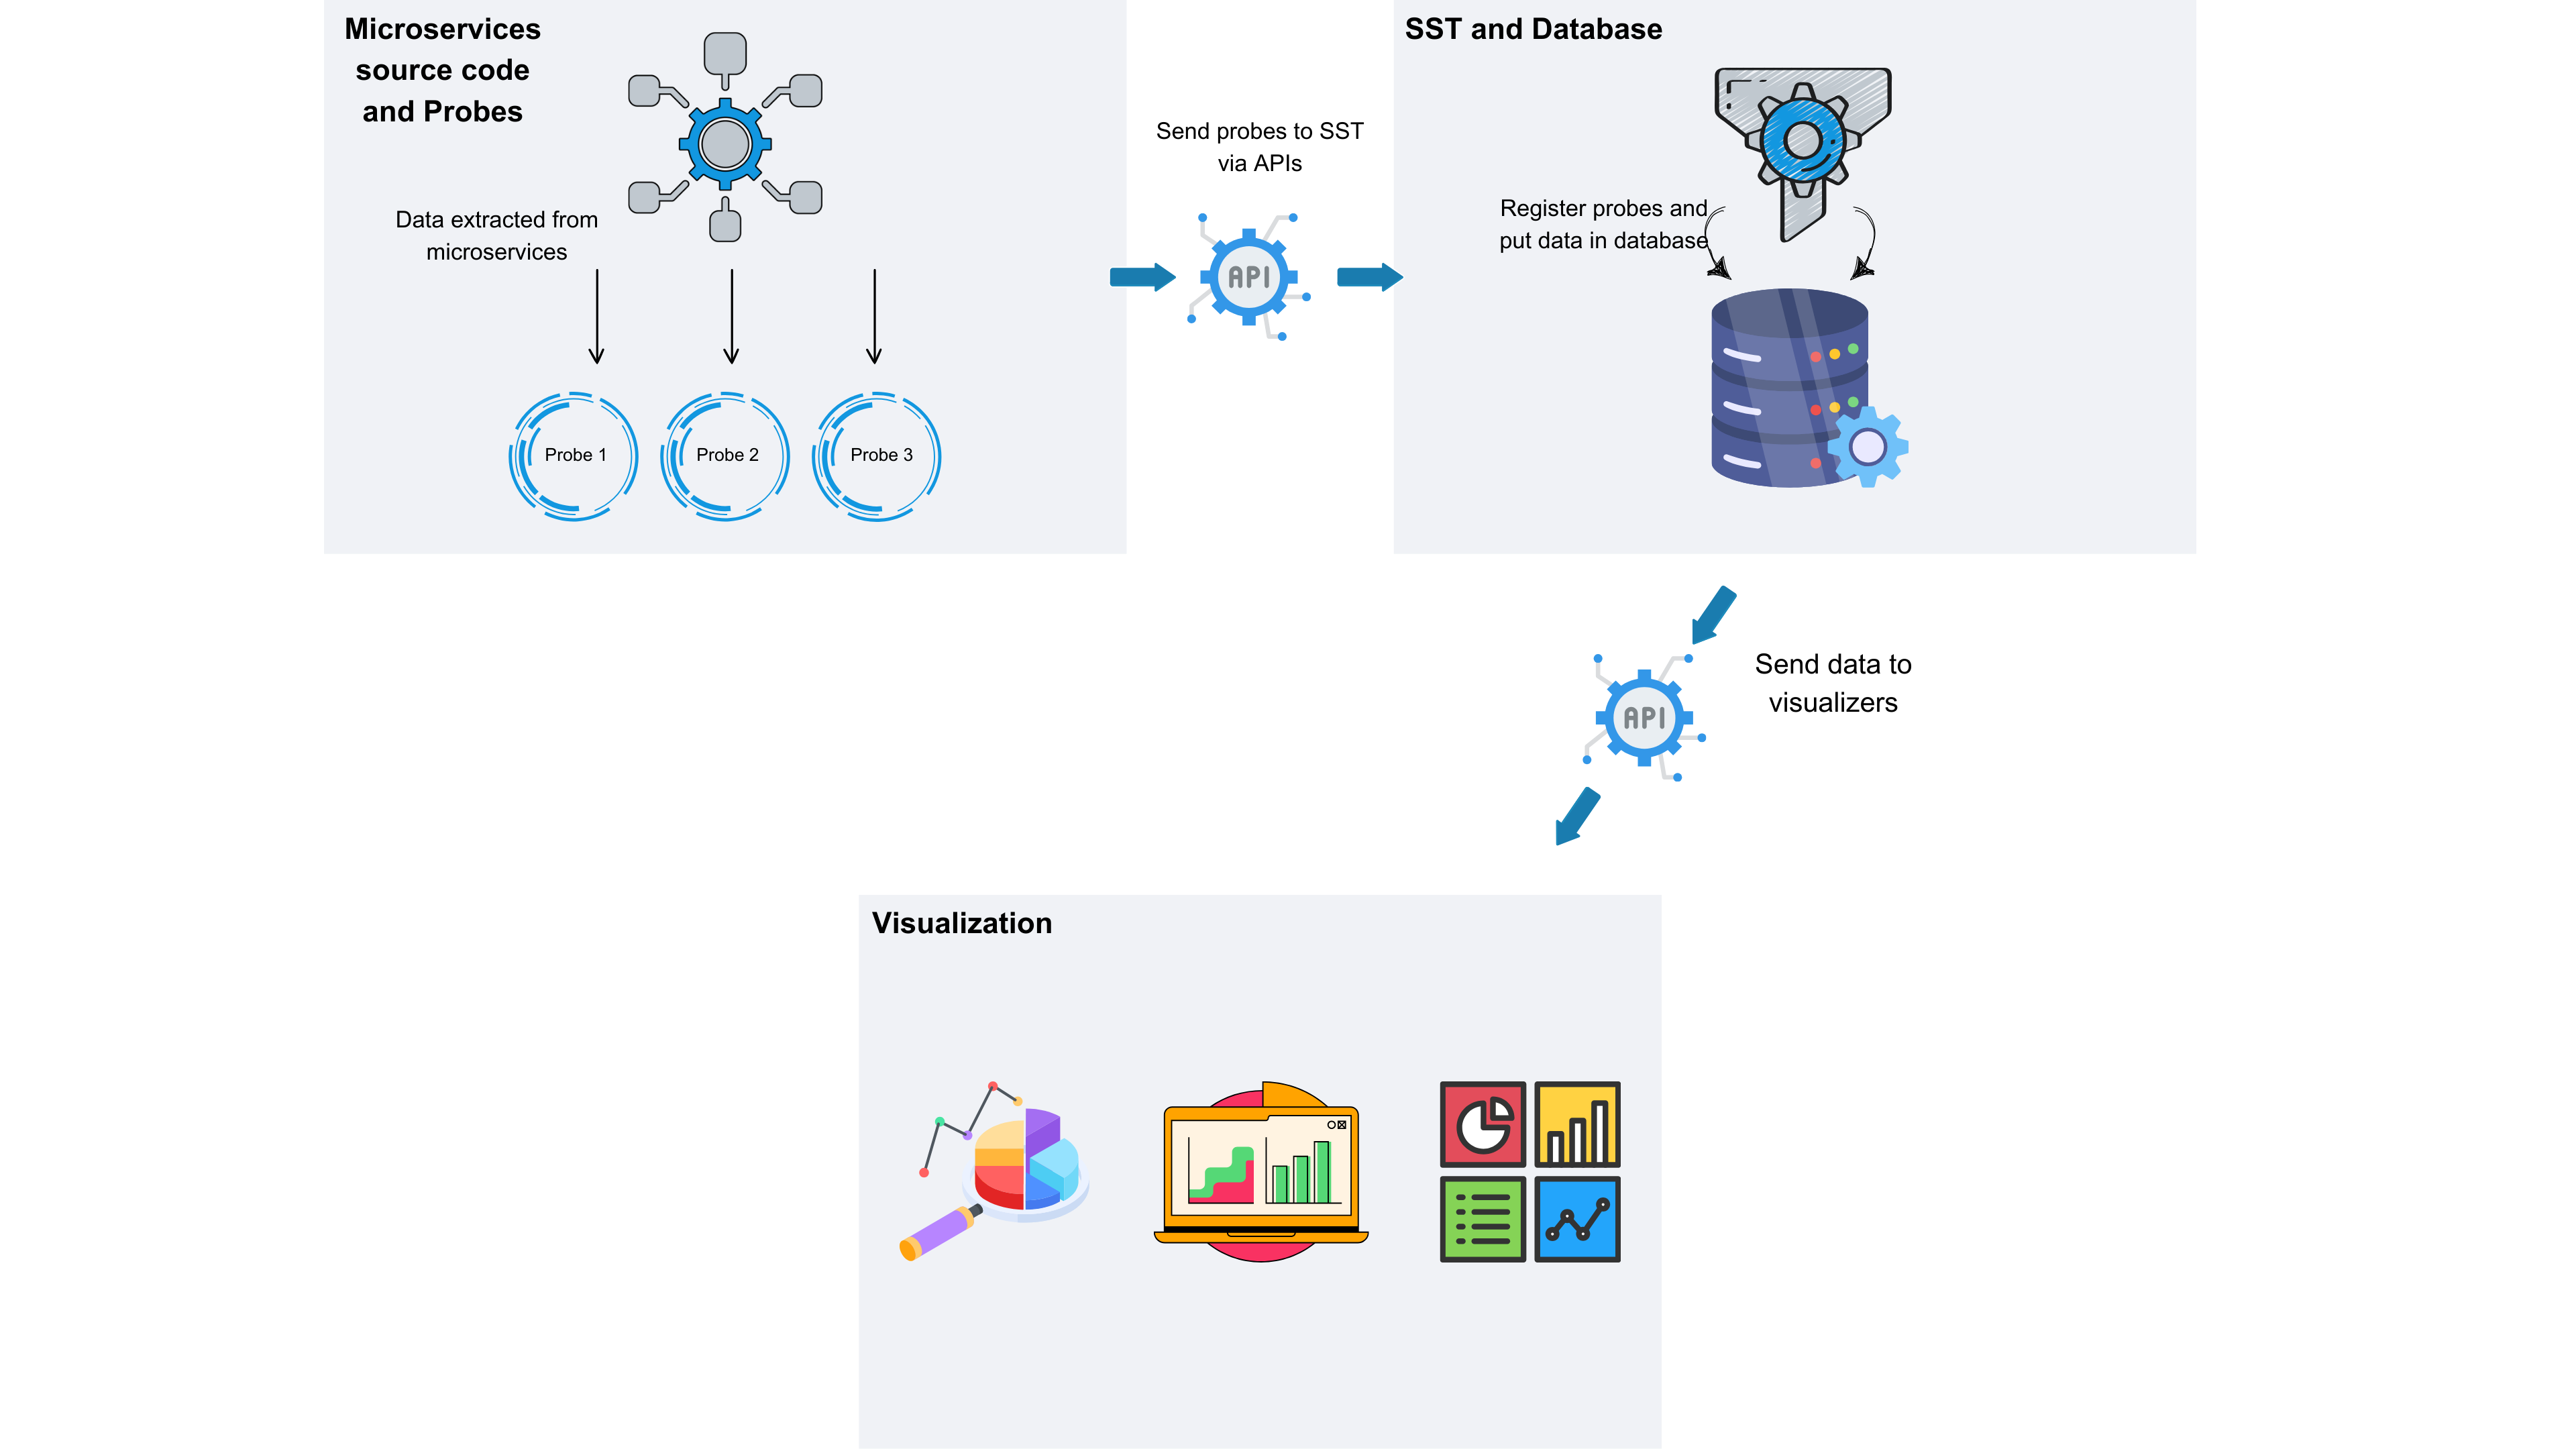
\includegraphics[width=1\textwidth]{figures/vision.png}
    \caption[Framework working]{Working of Probes, SST and Visualizer}
	\label{fig_vision}
\end{figure}

\section{Probes: Extractors}\label{sec:component-probes}

The first component of the framework consists of \textbf{probes}. Probes represent distinct informational artifacts that are systematically extracted from software systems to provide insights and actionable data. In the context of this report, we have several use cases to extract specific pieces of information that are detailed in the below subsections. These probes will help prove the framework credibility and serve as the foundational elements for gathering critical data points that enable analysis and decision-making. 

Looking forward, this concept can be expanded to more complex and targeted informational needs. By refining the scope and nature of the probes, we can tailor the probes according to our needs and to capture more refined data, addressing evolving requirements and insights that drive meaningful outcomes. This flexibility ensures that as the systems grow or change, the framework remains relevant and capable of producing deeper, more impactful information.

Given below are some of the probes use-cases as part of this report in order to show the credibility of the presented framework. In later chapters, their implementation will be discussed at length followed by the validation of each scenario discussed here.

\subsection{Authors Contributions}
The Author Contribution Probe is designed to extract detailed information about the developers involved in modifying a specific method. It identifies the developer who made the most recent changes, provides a list of all contributors to the method, and highlights the developer with the highest number of contributions.
\subsubsection{Use Cases:}
\begin{itemize}[label=$\bullet$]
	\item \textbf{Bug Fix}: When a bug is found in a method, the most recent author who updated the method would have the context of the recent changes that they have made and can help diagnose and resolve the issue faster. This will help the organization increase their productivity.
	\item \textbf{Reviews}: Looking at the most recent developer would give an idea of who to reach for documentation, clarification and review of the changes.
	\item \textbf{History Tracking}: Provides insights into who and why the person made the recent changes which can be used for documentation purposes.
	\item \textbf{Identify Developers Group}: Helps identify the group of developers who worked on a particular method, which in turn enables them to share and transfer knowledge in case the top contributor of the method is unavailable.
	\item \textbf{Ownership}: Tracks if the code has been worked on collaboratively or primarily by one individual.
	\item \textbf{Refactoring}: Ensures that all the contributors can be consulted and their insights are taken before performing any major refactoring.
	\item \textbf{Knowledge and Accountability}: Identifies the subject matter expert for particular methods and assigns ownership of the method to the top contributor for accountability and guidance.
	\item \textbf{Planning}: Helps management decide who should be involved in any major changes to the method based on past contributions.
\end{itemize}
\subsubsection{Benefits:}
\begin{itemize}[label=$\bullet$]
	\item \textbf{Improve Communication}: Facilitates and improve communication between team members by identifying relevant stakeholders.
	\item \textbf{Enhanced Planning}: Improves resource allocation, project planning and decision making for development tasks.
	\item \textbf{Transparency}: Promotes accountability among team members by making contribution history transparent.
	\item \textbf{Efficiency}: Increases team efficiency and issue resolving by involving right people for the job.
\end{itemize}

\subsection{File Authors}
This probe extracts information regarding the authors of a particular file. In software development, especially in large-scale microservices architecture, understanding the list of contributors to individual files provides significant value.
\subsubsection{Use Cases:}
\begin{itemize}[label=$\bullet$]
	\item \textbf{Ownership}: Identifying contributors of a particular file highlights the ownership and familiarity with the functionality of the file of the people associated with it.
	\item \textbf{Collaboration}: Identifying contributors reveals whether a file has been developed collaboratively or by a single individual.
	\item \textbf{Auditing and Compliance}: Contributor information is crucial for tracking accountability and compliance. Specially in open-source projects.
	\item \textbf{Maintenance}: Files with multiple contributors might lead to maintenance challenges. Having list of contributors help assign the tasks to the correct people.
	\item \textbf{Bug and Issue Assignment}: Assigning issues to contributors who are familiar with the relevant files improves resolution speed.
\end{itemize}
\subsubsection{Benefits:}
\begin{itemize}[label=$\bullet$]
	\item \textbf{Accountability and Quality}: Knowing who contributed to a file ensures accountability and encourages higher-quality contributions.
	\item \textbf{Team Collaboration}: Make team collaboration easier by identifying relevant stakeholders for discussions.
	\item \textbf{Reduces Risk}: Identifies files relying on single contributor which can help in workload distribution.
\end{itemize} 

\subsection{Author Relation}
This probe extracts information regarding the strength of collaboration between two authors. Greater the collaboration, great will be the strength of bond between them. The ``relation strength'' metric quantifies the level of collaboration between pairs of authors based on shared contribution to files. In collaborative software development, especially in microservices architectures, understanding the strength of relation among authors can provide valuable insights into teamwork, communication and collaboration in the development process.
\subsubsection{Use Cases:}
\begin{itemize}[label=$\bullet$]
	\item \textbf{Collaboration Analysis}: Provides a quantitative measure of collaboration between two developers in a development team. Higher strength shows frequent joint contributions.
	\item \textbf{Planning and Resource Allocation}: Helps plan tasks and form teams for future projects by using existing strong collaboration bonds.
	\item \textbf{Knowledge Transfer}: New developers can use relation strength data to identify key collaborators within the team.
	\item \textbf{Shared Ownership}: Helps determine the shared ownership of the files, making it easier to assign maintenance tasks.
	\item \textbf{Technical Debt}: Low pairwise strengths and high number of collaborators of a file represents cohesive ownership, leading to technical debt.
\end{itemize}
\subsubsection{Benefits:}
\begin{itemize}[label=$\bullet$]
	\item \textbf{Improved team dynamics}: Improve team dynamics and encourages better interaction in areas with weaker team collaboration.
	\item \textbf{Fast Problem Solving}: Developers with high collaboration strength are likely to solve issues in shared files effectively.
	\item \textbf{Transparency}: Visualizes team interactions, increasing accountability and transparency.
	\item \textbf{Employee Evaluation}: Management can use the data to evaluate employees. Developers with higher collaboration strengths with multiple individuals shows employee value.
\end{itemize} 

\subsection{Microservices Endpoints}
This probes extracts REST API endpoints from each service of a microservices project. Extracting such data provide valuable insights into how the application communicates and interacts with external systems or clients.
\subsubsection{Use Cases:}
\begin{itemize}[label=$\bullet$]
	\item \textbf{Documentation and Analysis}: Automatically extracts endpoints information to generate accurate and up-to-date documentation and perform analysis.
	\item \textbf{Application Functionality}: Provides overview of the functionality exposed by each service.
	\item \textbf{Testing}: Extracted endpoint data can be used to perform regression testing and prioritize test cases.
	\item \textbf{Security Audits}: Endpoint extraction aids in auditing APIs for potential security vulnerabilities.
	\item \textbf{Productivity}: Helps developers understand the microservices quicks and API offerings of each service.
\end{itemize}
\subsubsection{Benefits:}
\begin{itemize}[label=$\bullet$]
	\item \textbf{Debugging Issues}: Helps locating the faulty file and class, and helps developers quickly identify the method handling the request and resolve the issue.
	\item \textbf{Documentation}: Teams can use extracted endpoint data providing clients with API documentation.
	\item \textbf{Collaborations}: Facilitates communication between backend and frontend teams by providing endpoint insights.
\end{itemize} 

\subsection{Spring Beans}
This probe extracts beans from java spring framework services. In Spring, the objects that form the backbone of your application and that are managed by the Spring IoC container are called beans. A bean is an object that is instantiated, assembled, and managed by a Spring IoC container. Otherwise, a bean is simply one of many objects in your application. Beans, and the dependencies among them, are reflected in the configuration metadata used by a container~\citep{spring_beans_intro}.
\subsubsection{Use Cases:}
\begin{itemize}[label=$\bullet$]
	\item \textbf{Debugging and Maintenance}: Bean extraction provides a clear map of all components, aiding in debugging and maintenance activities.
	\item \textbf{Debugging and Maintenance}: Extracted bean data reveals the dependencies between components, helping teams understand coupling within the application.
	\item \textbf{Dynamic Bean Management}: Helps to enable dynamic and conditional bean registration and configuration.
\end{itemize}
\subsubsection{Benefits:}
\begin{itemize}[label=$\bullet$]
	\item \textbf{Improves Debugging}: Quickly locates missing or misconfigured beans, reducing the development downtime.
	\item \textbf{Security Improvement}: Detects potential security risks and stability issues.
\end{itemize} 

\subsection{Extracting Dependencies}
This probe extracts dependencies from the POM (Project Object Model) files. A POM (Project Object Model) file is an XML file that serves as the fundamental building block of a Maven project. It contains information about the project and configuration details to manage dependencies, plugins, build settings, and more~\citep{pom_file_guide}.
\subsubsection{Use Cases:}
\begin{itemize}[label=$\bullet$]
	\item \textbf{Dependency Management and Version Control}: Extracting dependencies helps track the versions of libraries and frameworks used across microservices.
	\item \textbf{Microservices Dependencies}: Analyze dependencies to understand the relationships between microservices and their shared libraries.
	\item \textbf{Performance Optimization}: Shows performance heavy libraries or those that introduce inefficiencies.
\end{itemize}
\subsubsection{Benefits:}
\begin{itemize}[label=$\bullet$]
	\item \textbf{Improves Performance}: Helps to identify, update or remove unused dependencies optimizing the performance and efficiency of the services.
	\item \textbf{Security Improvement}: Make it easy to identify those dependencies that are impacting the security of the services.
	\item \textbf{Maintainability}: Help keep all the dependencies up-to-date and easy to maintain.
\end{itemize} 

\section{Single Source of Truth (SST)}\label{sec:component-sst}

When data is being extracted from different sources, there are high chances of it becoming inconsistent and stale. If some sort of analysis is being done on the data, the input data needs to be up-to-date and reliable. In section~\ref{sec:vision} (\nameref{sec:vision}), we mentioned the visualizer component. It is supposed to run desired analysis on the data and provide visual updates. More on the visualizer in the upcoming subsection. So, if analysis is to be done on the input data, it needs to be a trusted, accessible, credible, reliable, and consistent.

Maintaining data quality is crucial for accurate insights and decision-making. Unified sources ensure that the input data remains clean and updated, regardless of its origin. Properly validated and processed data serves as the foundation for meaningful analysis and visualization.

\citep{MullerUdsforSA2018} presents a scalable and extensible approach for software analysis and visualization by integrating data from diverse sources into a unified source. The paper discusses that having a unified data source provides a single access point for querying diverse data, eliminating the need to manage multiple disconnected sources. 

The single source of truth (SST) component in the introduced framework does the same job as a unified data source. It is working as a data warehouse that takes all the information from different artifacts and process it. The tool used as a single source of truth in this project will be discussed in chapter 4 (~\nameref{chap:implementation_report}) and the validation of the output provided will be discussed in chapter 5 (~\nameref{chap:scenario_validations}).

\begin{figure}[H]
    \centering
    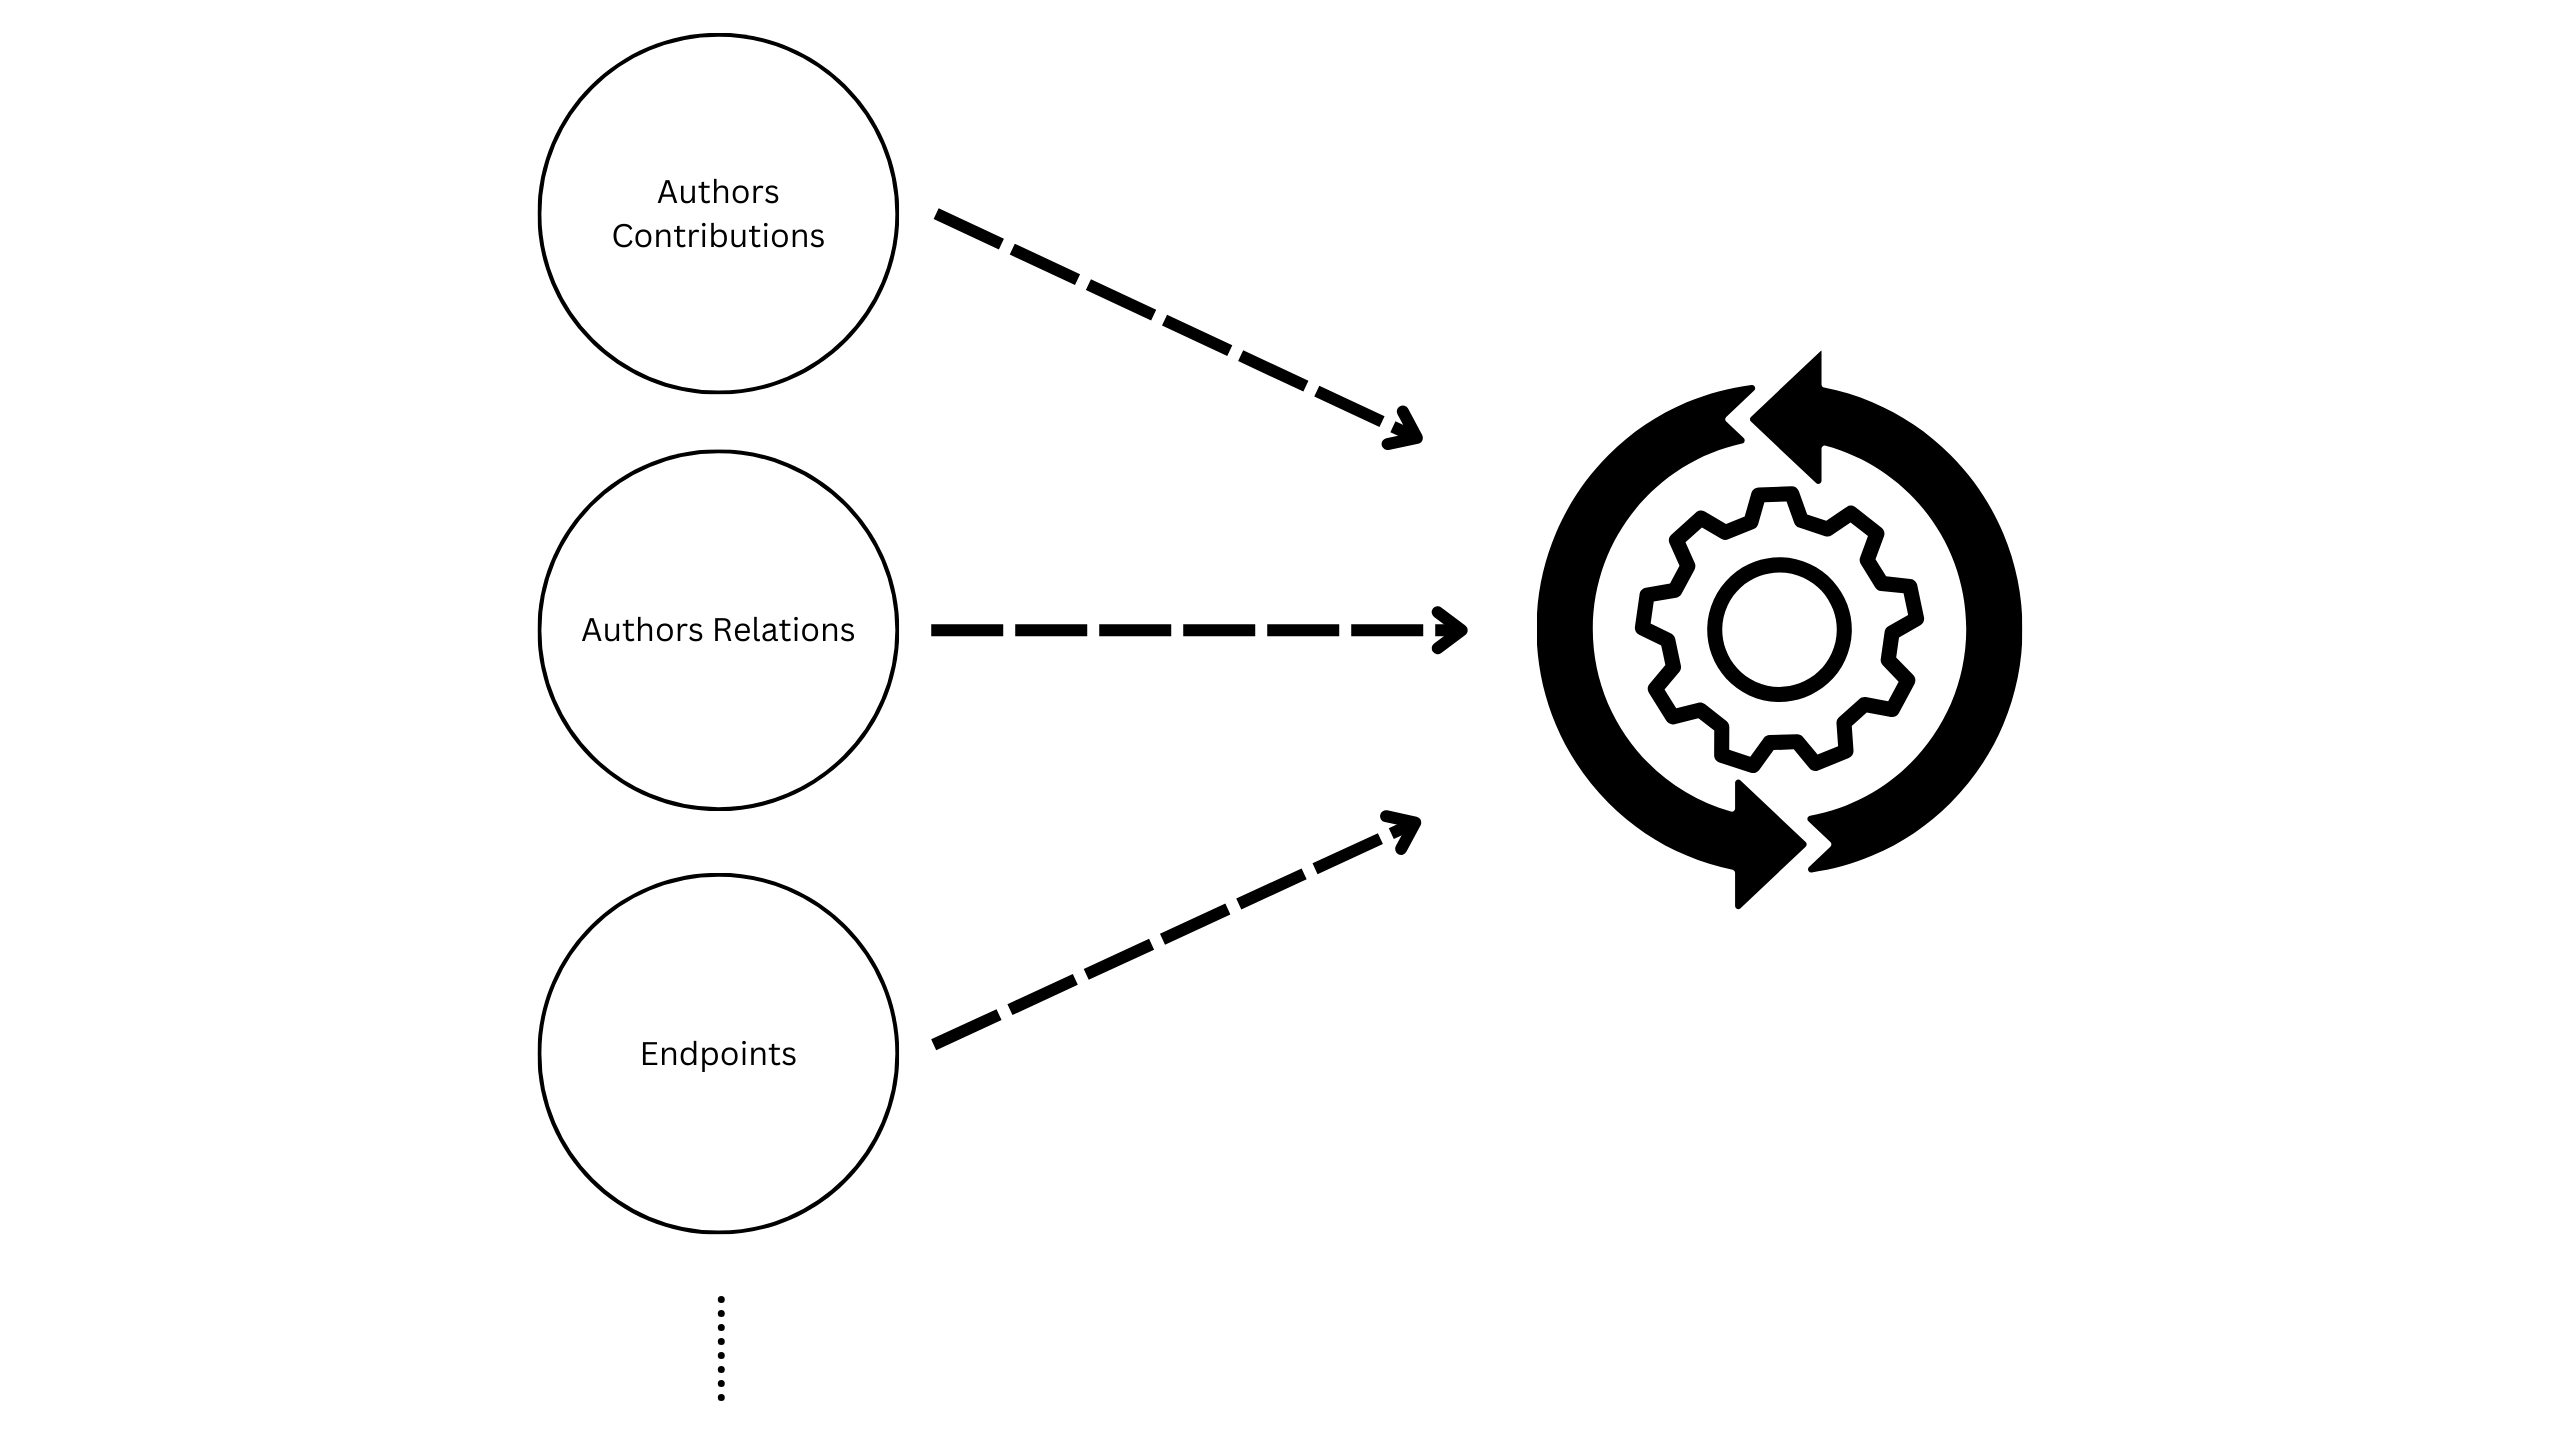
\includegraphics[width=1\textwidth]{figures/sst_working.png}
    \caption[Probes and SST]{Probes and SST}
    \label{fig_probes_sst}
\end{figure}

\subsection{Integration and Output}

The probes will extract the required data from the microservices and feed them to the SST for further processing. SST will generate output which will be used by the visualizer for further analysis and visualization.

\subsection{Data Management}

The output of the SST will be stored in a separate database to maintain and preserve historical records systematically. This approach ensures that the data is structured, organized, and easily retrievable from a centralized repository. By consolidating the data into a single repository, it not only simplifies access but also ensures a consistent format, which is critical for long-term usability and reliability. 

Storing the data in a database enhances its integrity by eliminating inconsistencies and reducing complexities, such as duplicate entries. This structure allows analysts or analysis tools to focus on extracting meaningful insights without the additional work of cleaning or reorganizing raw data.

Additionally, a dedicated database supports scalability, meaning it can accommodate larger datasets as the system evolves. It also offers improved data management capabilities, such as access controls and backup solutions, ensuring the data remains protected and readily available for future use.

\section{Visualizer}\label{sec:component-visualizer}

After software analysis is completed with the help of probes and SST, we can use some visualizer tools in order to produce useful information gathered from the software system. There are bunch of tools that are already available provided by different software companies or we can create our own system in order to visualize the data as per need. 

There are diverse range of software visualization and analysis tools available in the market, with each of them having their own strengths and weaknesses.~\citep{SWVizTools2001} covers more than 40 tools for software visualization with each having their own advantages. For example, Rigi is used for understanding legacy system, GraphViz is popular for graph-based visualizations and daVinci offers dynamic graph layouts.

Following are some of the important tools offered by AWS and Azure for visualization.
\begin{itemize}[label=$\bullet$]
	\item \textbf{Amazon QuickSight}: A business intelligence (BI) service that enables users to visualize data through dashboards, interactive graphs, and analytics. It connects to various data sources, including software systems, databases, and AWS services and perform real-time data analysis. Read more about this from~\citep{AWSQuickSight2025}. 
	\item \textbf{Amazon X-Ray}: A service for analyzing and debugging applications. It collects data about requests to your applications, including errors and performance bottlenecks. Visualizes the application architecture in a service map for easy identification of issues. Read more about this from~\citep{AWSXRay2025}.
	\item \textbf{Azure Monitor}: Azure monitor collects, analyzes, and visualizes telemetry data from azure and on-premise environments to monitor application performance and detect issues. Key features are logs and metrics collection for in-depth analysis, provides alerts and insights to troubleshoot issues in real-time etc. Read more from ~\citep{AzureMonitor2025}.
	
	\begin{figure}[H]
		\centering
		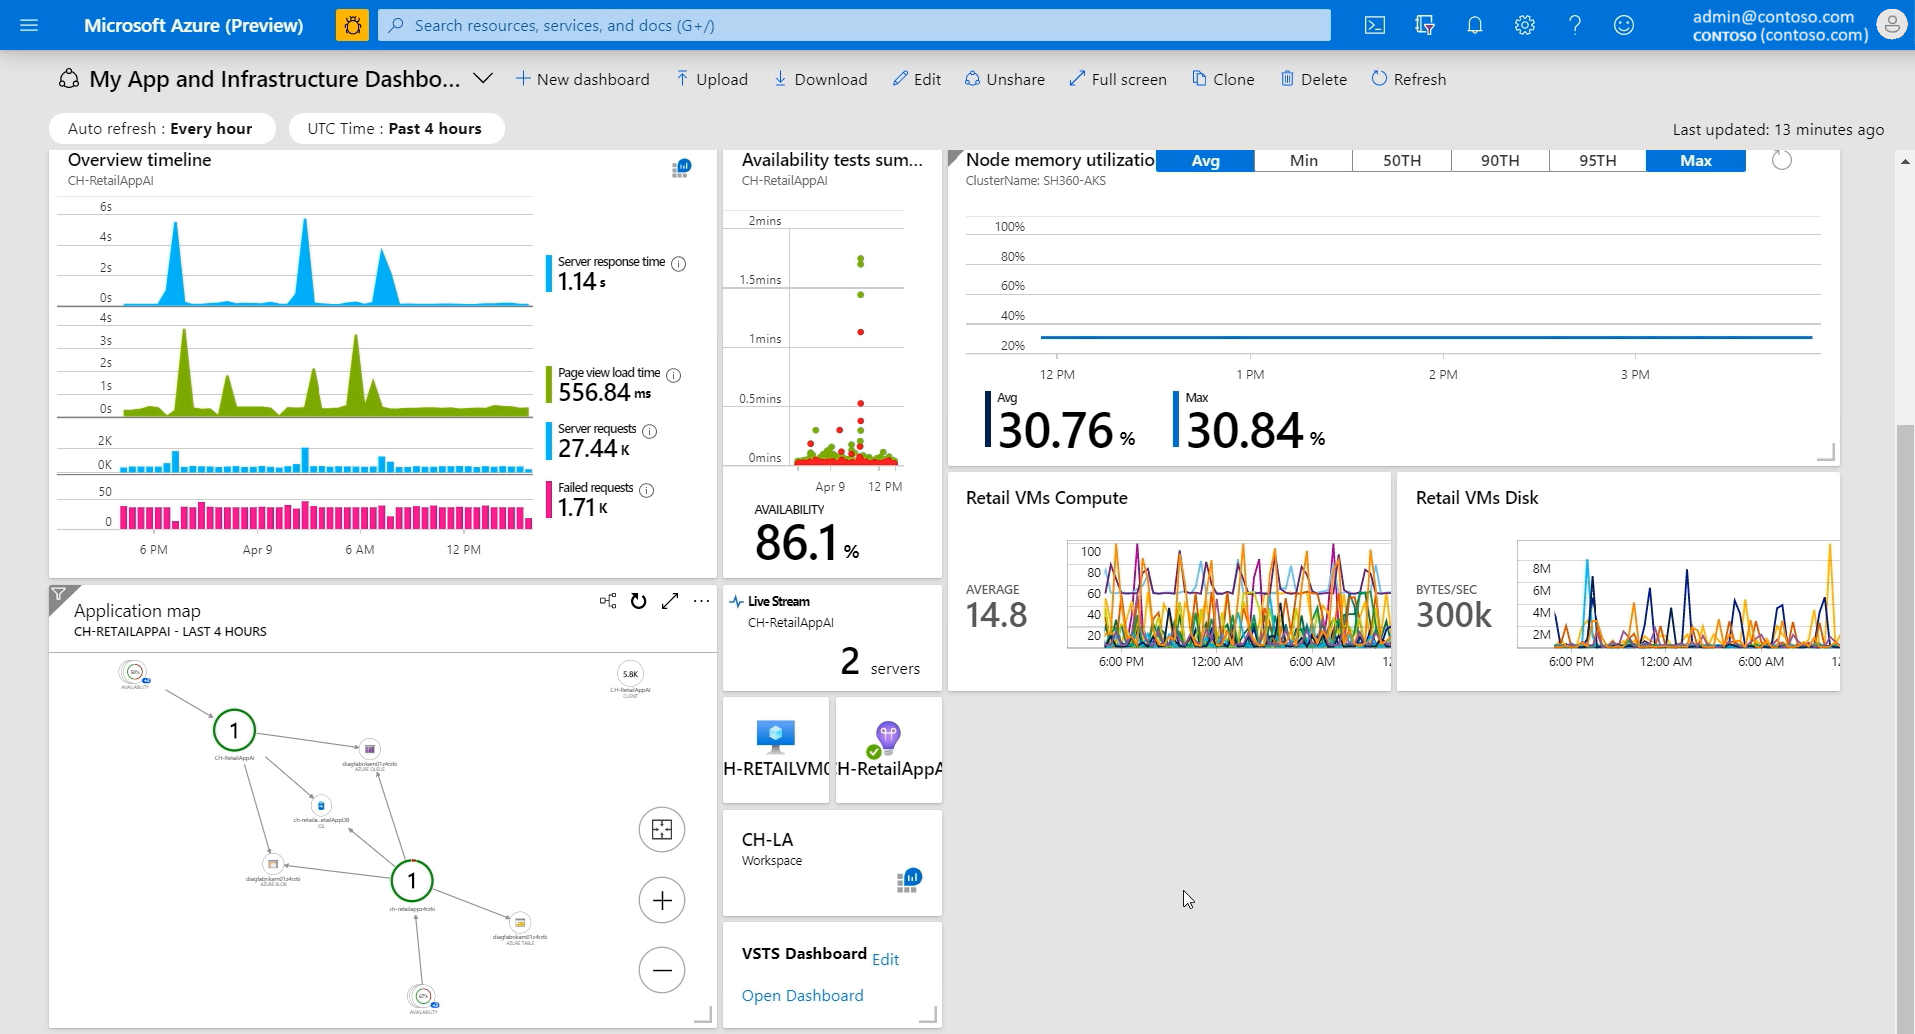
\includegraphics[width=0.9\textwidth]{figures/azure_monitor_dashboard.png}
		\caption[Azure Monitor]{Dashboard of Azure monitor (adapted from~\cite{AzureMonitorBestPractices2025})}
		\label{fig_azure_monitor}
	\end{figure}

\end{itemize}


In our report, once the probes and SST are integrated, the processed data from SST will be used in for the visualization of data produced by the above mentioned probes. 

\section{Referencing}
These are some sample references to GAMYGDALA~\citep{popescu2014gamygdala} from 
the \texttt{references.bib} file and state effects of 
cognition~\citep{hudlicka2002time} from the \texttt{references\_another.bib} 
file. These references are not in the same .bib file.

\section{Figures}
This is a single image figure (Figure~\ref{fig_singleenv}):

\begin{figure}[ht]
    \centering
    
\includegraphics[width=0.6\textwidth]{figures/Sample/tumblr_static_eaceks0rfxsss8o4swscw40wo.jpg}
    \caption[Single Figure Environment Listed Title]{This is a single figure 
    environment}
    \label{fig_singleenv}
\end{figure}

This is a multi-image figure with a top (Figure~\ref{fig_multienv_1}) and bottom (Figure~\ref{fig_multienv_2}) aligned subfigures:

\begin{figure}[ht]
	\centering
	\begin{subfigure}[t]{\textwidth}
		\centering
		

\includegraphics[width=0.7\textwidth]{figures/Sample/tumblr_static_eaceks0rfxsss8o4swscw40wo.jpg}
		\caption{Figure 1}
		\label{fig_multienv_1}
	\end{subfigure}
	~
	\begin{subfigure}[t]{\textwidth}
		\centering
		

\includegraphics[width=0.7\textwidth]{figures/Sample/tumblr_static_eaceks0rfxsss8o4swscw40wo.jpg}
		\caption{Figure 2}
		\label{fig_multienv_2}
	\end{subfigure}
	
	\caption{A Multi-Figure Environment}
	\label{fig_multienv}
\end{figure}

\section{Tables}

Here is a sample table (Table~\ref{tab_sample}):

	\begin{table}[ht]
	\centering
	\begin{tabular}{ m{0.2\textwidth} m {0.1\textwidth} m{0.15\textwidth} }
		\toprule
		A & $\longleftrightarrow$ & B \\
		C & $\longleftrightarrow$ & D \\
		\bottomrule	
	\end{tabular}	
	\caption{A sample table}	
	\label{tab_sample}
\end{table}

\subsection{Long Tables}
A sample long table is shown in Appendix~\ref{appendix_b}.

\section{Equations}

Here is a sample equation (Equation~\ref{eq_lineslope}):

\begin{equation} \label{eq_lineslope}
	y = mx + b
\end{equation}